\vspace{-.5em}
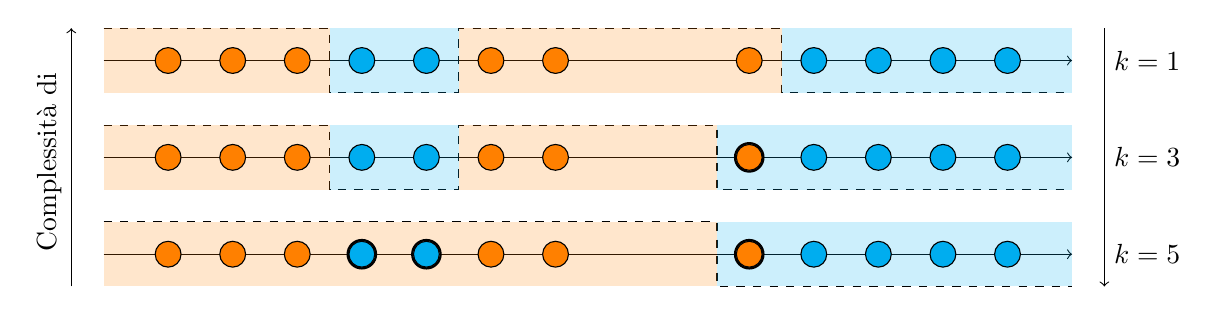
\begin{tikzpicture}[scale=.82]
    
    \def \r {.2}
    
    \draw[->] (0,3) -- (15,3);
    \draw[->] (0,1.5) -- (15,1.5);
    \draw[->] (0,0) -- (15,0);

    \draw[dashed] (0,3.5)--(3.5,3.5)--(3.5,2.5)--(5.5,2.5)--(5.5,3.5)
        --(10.5,3.5)--(10.5,2.5)--(15,2.5);
    \fill[orange, opacity=.2] (0,3.5)   rectangle (3.5,2.5);
    \fill[orange, opacity=.2] (5.5,3.5) rectangle (10.5,2.5);
    \fill[cyan  , opacity=.2] (3.5,3.5) rectangle (5.5,2.5);
    \fill[cyan  , opacity=.2] (10.5,3.5) rectangle (15,2.5);

    \draw[dashed] (0,2)--(3.5,2)--(3.5,1)--(5.5,1)--(5.5,2)
        --(9.5,2)--(9.5,1)--(15,1);
    \fill[orange, opacity=.2] (0   ,2) rectangle (3.5 ,1);
    \fill[orange, opacity=.2] (5.5 ,2) rectangle (9.5,1);
    \fill[cyan  , opacity=.2] (3.5 ,2) rectangle (5.5 ,1);
    \fill[cyan  , opacity=.2] (9.5,2) rectangle (15  ,1);

    \draw[dashed] (0,.5)--(9.5,.5)--(9.5,-.5)--(15,-.5);
    \fill[orange, opacity=.2] (0  ,.5) rectangle (9.5,-.5);
    \fill[cyan  , opacity=.2] (9.5,.5) rectangle (15 ,-.5);

    \draw[thick] (10,1.5) circle (\r+.02);
    \draw[thick] (4 ,0)   circle (\r+.02);
    \draw[thick] (5 ,0)   circle (\r+.02);
    \draw[thick] (10,0)   circle (\r+.02);

    \foreach \y in {3,1.5,0} {
        \draw[fill=orange] (1, \y) circle (\r);
        \draw[fill=orange] (2, \y) circle (\r);
        \draw[fill=orange] (3, \y) circle (\r);
        \draw[fill=cyan]   (4, \y) circle (\r);
        \draw[fill=cyan]   (5, \y) circle (\r);
        \draw[fill=orange] (6, \y) circle (\r);
        \draw[fill=orange] (7, \y) circle (\r);
        \draw[fill=orange] (10,\y) circle (\r);
        \draw[fill=cyan]   (11,\y) circle (\r);
        \draw[fill=cyan]   (12,\y) circle (\r);
        \draw[fill=cyan]   (13,\y) circle (\r);
        \draw[fill=cyan]   (14,\y) circle (\r);
    }
    
    \draw[->] (-.5,-.5) -- (-.5,3.5);
    \node[rotate=90,above] at (-.5,1.5) {Complessità di $\hknn$};
    \draw[->] (15.5,3.5) -- (15.5,-.5);
    \node[right] at (15.5,3)   {$k=1$};
    \node[right] at (15.5,1.5) {$k=3$};
    \node[right] at (15.5,0)   {$k=5$};

\end{tikzpicture}
\vspace{-.5em}